\section{Prune}

\subsection{Observation}
\begin{frame}
    \frametitle{Observation}
	\begin{figure}
		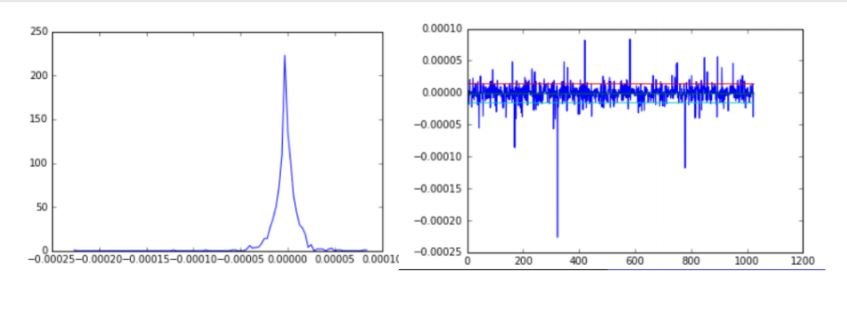
\includegraphics[scale=0.4]{figure/gradient_observation.JPG}
	\end{figure}
\end{frame}


\subsection{Prune}
\begin{frame}
    \frametitle{Prune}
    \begin{itemize}
		\item Prune gradients: Send gradients which are absolutely greater than threshold. 
			\begin{itemize}
				\item Static threshold: 10\%, 1\%, 0.1\%. 
				\item Standard deviation threshold: 1, 2, 3. 
				\item Dynamic threshold: mean of the gradients which are greater than last threshold. 
			\end{itemize}
	\end{itemize}
\end{frame}

\subsection{Standard deviation threshold}
\begin{frame}
	\frametitle{Standard deviation threshold}
	\begin{itemize}
		\item Compute standard deviation on gpu. 
		\item Faster 30 times than cpu.
		\item Use 25\% computation time. 
	\end{itemize}
\end{frame}
\begin{frame}
    \frametitle{experiment 1}
	\begin{figure}
		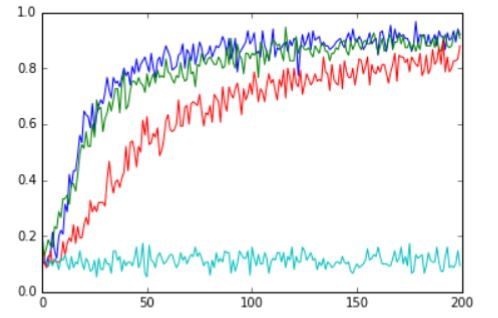
\includegraphics[scale=0.4]{figure/stdexp1.JPG}
	\end{figure}
\end{frame}

\begin{frame}
    \frametitle{experiment 2}
	\begin{itemize}
		\item To do: accuracy for each time. 
	\end{itemize}
\end{frame}

\subsection{Static threshold}
\begin{frame}
	\frametitle{Static threshold}
	\begin{itemize}
		\item Compute on gpu. 
		\item Selection algorithm. 
	\end{itemize}
\end{frame}
\begin{frame}
    \frametitle{experiment 1}
	\begin{itemize}
		\item To do: accuracy for each interation. 
	\end{itemize}
\end{frame}

\begin{frame}
    \frametitle{experiment 2}
	\begin{itemize}
		\item To do: accuracy for each time. 
	\end{itemize}
\end{frame}
\subsection{Dynamic threshold}
\begin{frame}
	\frametitle{Dynamic threshold}
	\begin{itemize}
		\item Compute on gpu. 
		\item Next threshold = mean of the gradients which are greater than current threshold
	\end{itemize}
\end{frame}
\begin{frame}
    \frametitle{experiment 1}
	\begin{itemize}
		\item To do: accuracy for each interation. 
	\end{itemize}
\end{frame}

\begin{frame}
    \frametitle{experiment 2}
	\begin{itemize}
		\item To do: accuracy for each time. 
	\end{itemize}
\end{frame}

